% directories with graphics
\graphicspath{{../gfx/}}
\DeclareGraphicsExtensions{.pdf,.png,.jpg}

% TikZ libraries
\usetikzlibrary{
  % arrow types
  arrows.meta,
  % for background grids as navigational aid
  backgrounds,
  % coordinate calculations
  calc,
  % torn paper effect,
  decorations.pathmorphing,
  % curly braces
  decorations.pathreplacing,
  % text along path
  decorations.text,
}

% suppress pgfplots "backwards compatibility" warning
\pgfplotsset{compat=1.15}

% set default line width to same as in Matplotlib plots
% created by helper.figure
\tikzset{every picture/.style={line width=1pt}}

% set default arrow tip
\tikzset{>={Stealth[length=5.5pt,width=5.5pt]}}

% draw circle arc around center (standard in TikZ is
% the specification of the first point on the arc)
% [draw options] (center) (initial angle:final angle:radius)
\def\centerarc[#1](#2)(#3:#4:#5){
  \draw[#1] ($(#2)+({(#5)*cos(#3)},{(#5)*sin(#3)})$) arc (#3:#4:#5);
}

% dotted lines with round dots
% use with \draw[->,dots] (node1) to (node2);
\tikzset{
  dot diameter/.store in=\dot@diameter,
  dot diameter=0.8mm,
  dot spacing/.store in=\dot@spacing,
  dot spacing=1.4mm,
  dots/.style={
    line width=\dot@diameter,
    line cap=round,
    dash pattern=on 0pt off \dot@spacing
  }
}

% text along path
\tikzset{
  textalongpath/.style 2 args={
    decoration={
      text align={left indent=#1},
      text along path,
      text={#2}
    },
    decorate
  }
}

% insert circle with section title
\newcommand*{\sectionCircle}{
  \fill[mittelblau] (80,-20) circle (60mm);
  \node[
    white,
    anchor=center,
    align=center,
    text width=100mm,
  ] at (80,15) {\huge\textbf{\insertsection}};
}

% insert circle with subsection title, arguments:
% {x coordinate}{y coordinate}{title}{highlight? 0 or 1}
\newcommand*{\subsectionCircle}[4]{
  \fill[hellblau,anchor=center] (#1,#2) circle (18mm);
  \ifnum#4>0
    \draw[red] (#1,#2) circle (18mm);
  \fi
  \node[
    white,
    text width=36mm,
    align=center,
    anchor=center,
    font=\bfseries,
  ] at (#1,#2) {#3};
}

% excerpt from thesis as rotated circle, arguments:
% {x coordinate on slide}{y coordinate on slide}{radius on slide}
% {x coordinate on page}{y coordinate on page}{radius on page}{page no.}
\newcommand*{\thesisCircle}[7]{
  {
    \transparent{0.4}
    \fill[black] ($({#1+1mm},{#2-1mm})$) circle (#3+0.5mm);
  }
  \node[thesis circle={#3}{#4}{#5}{#6}{#7}] at (#1,#2) {};
}

\newlength{\tcleft}
\newlength{\tcbottom}
\newlength{\tcright}
\newlength{\tctop}
\newlength{\tcwidth}
\newcommand*{\tcangcon}{0}
\tikzset{
  thesis circle/.style n args={5}{
    circle,
    anchor=center,
    draw=mittelblau,
    fill=mittelblau!20,
    minimum size=2*#1,
    inner sep=0mm,
    path picture={
      \node[anchor=center,rotate=\tcangcon] at (0,0) {%
        \def\tcpage{\numexpr#5+2\relax}%
        \pgfmathsetlength{\tcleft}{#2-#4}%
        \pgfmathsetlength{\tcbottom}{297mm-(#3+#4)}%
        \pgfmathsetlength{\tcright}{210mm-(#2+#4)}%
        \pgfmathsetlength{\tctop}{#3-#4}%
        \pgfmathsetlength{\tcwidth}{2*#1}%
        \includegraphics[
          page=\tcpage,
          trim={\tcleft{} \tcbottom{} \tcright{} \tctop{}},
          clip,
          width=\tcwidth,
        ]{thesis}%
      };
    }
  }
}

% caption for \thesisCircle, arguments:
% {x coordinate on slide}{y coordinate on slide}{radius on slide}
% {start angle}{end angle}{text}
\newcommand*{\thesisCircleCaption}[6]{
  \ifnum#4<#5
    \def\tccradius{0.35em}
  \else
    \def\tccradius{1.0em}
  \fi
  \begin{scope}[xshift=#1,yshift=#2]
    \fill[mittelblau]
      ($({(#3-1.3em)*cos(#4)},{(#3-1.3em)*sin(#4)})$) --++ (0,0) arc[
        start angle=#4,
        end angle=#5,
        radius=#3-1.3em,
      ] -- ($({(#3)*cos(#5)},{(#3)*sin(#5)})$) --++ (0,0) arc[
        start angle=#5,
        end angle=#4,
        radius=#3,
      ] -- cycle;
    \path[
      postaction={decorate},
      decoration={
        text along path,
        text align=center,
        text={|\color{white}|#6},
      },
    ] ($({(#3-\tccradius)*cos(#4)},{(#3-\tccradius)*sin(#4)})$) arc[
      start angle=#4,
      end angle=#5,
      radius=#3-\tccradius,
    ];
  \end{scope}
}
